\begin{wrapfigure}{r}{0.5\textwidth}
  \vspace{-30pt}
  \begin{center}
    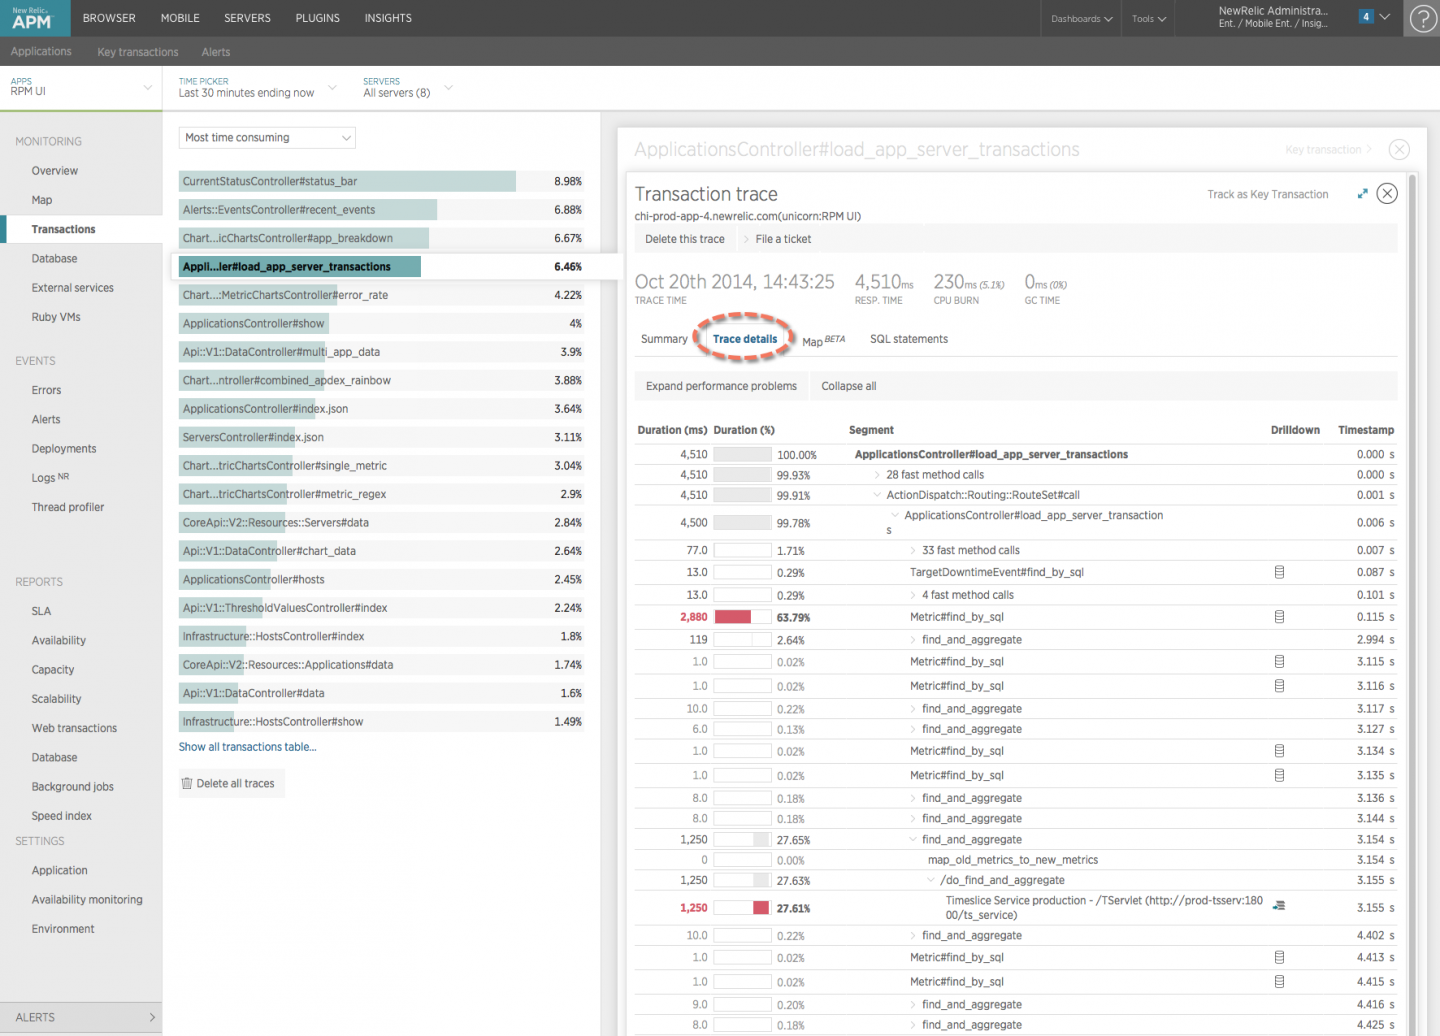
\includegraphics[width=0.48\textwidth]{images/new-relic_trace}
  \end{center}
  \vspace{-22pt}
  \caption{\emph{New Relic} - exemple de trace}
  \vspace{-20pt}
\end{wrapfigure}

\emph{New Relic} est un outil disponible en mode \gls{SaaS} permettant de surveiller les serveurs de \gls{production} tout en ayant un impact négligeable sur les performances.

Il propose différentes fonctionnalités dont notamment une permettant d'afficher, sous forme de trace, des \glspl{metrique} sur le code exécuté. Il va ainsi permettre d'afficher une trace, un profil du code exécuté, avec le temps passé dans chaque fonction.
 
\clearpage
Cet outil est intéressant sur plusieurs points :
\begin{itemize}
  \item Le langage \Python est supporté
  \item L'expérience utilisateur est proche de celle de \Blackfire (pas ou peu d'instrumentation manuelle requise)
\end{itemize}
  
Enfin le code source du module de l'agent \emph{New Relic} pour \Python est disponible sur \gls{PyPI}\footnote{\url{https://pypi.python.org/pypi/newrelic}}, ce qui permet de comprendre son fonctionnement.
  
  \subsubsection{Collecte des métriques}
Pour collecter le \gls{graphe d'appels} et les temps associés, deux techniques sont misent en œuvre en parallèle. \\
D'un côté l'agent va lancer un thread spécial qui sera chargé de récupérer la \gls{pile d'appels} à intervalle régulier et de l'utiliser pour reconstituer le \gls{graphe d'appels} du programme. \\
De l'autre diverses méthodes et fonctions estimées importantes sont décorées afin de récupérer plus d'information comme le temps d'exécution ou la requête SQL exécutée.

Cette instrumentation se fait en plusieurs étapes \footnote{Voir Annexe \vref{app:newrelicdecorationmethodes} pour le code correspondant} :
\begin{enumerate}
  \item Définition d'un \emph{\gls{chargeur de modules}} personnalisé afin de décorer automatiquement les modules quand ils sont chargés.
  \item Lecture dans le fichier de configuration de la liste des méthodes à décorer.
  \item Enregistrement d'un \emph{\gls{hook}} pour chacune des méthodes à décorer auprès du chargeur de modules.
  \item Lors du chargement d'un module, le chargeur de modules va exécuter tous les hooks se rapportant au module en question afin d'en décorer les méthodes.
\end{enumerate}

Cette instrumentation fonctionne à partir d'un fichier de configuration indiquant quelles méthodes doivent être instrumentées ; elle est donc parfaitement générique. En outre, le fait de n'instrumenter qu'une partie des appels de fonctions permet de limiter l'impact du profileur au point d'en être négligeable, surtout qu'il existe une librairie\footnote{\url{https://pypi.python.org/pypi/wrapt}} (écrite dans le langage C) permettant de décorer facilement et à moindre coût n'importe quelle fonction ou méthode \emph{Python}.
